\documentclass[a4paper, 12pt]{article}
\usepackage[portuges]{babel}
\usepackage{amsmath,amssymb,amsfonts,amsthm} 
\usepackage{indentfirst}
\usepackage{graphicx}
\usepackage[colorinlistoftodos]{todonotes}
\usepackage{verbatim}
\usepackage{textcomp}
\usepackage{csquotes}
\usepackage{gensymb}
\usepackage{biblatex}
\addbibresource{bibliografia.bib}
\usepackage[a4paper,top=3cm,bottom=2cm,left=3cm, right=2cm]{geometry}
\usepackage{indentfirst}
\usepackage{float}
\usepackage{multicol}
\usepackage{multirow}
\usepackage{graphicx}
\usepackage{anyfontsize}
\usepackage{setspace}
\usepackage[titles]{tocloft}
\usepackage{fontspec}
\usepackage{fancyhdr}
\usepackage{newfloat}
\usepackage{tabls}
\usepackage{makecell}
\usepackage{shadowtext}
\usepackage{eso-pic,graphicx}
\usepackage{tikz}
\usepackage[absolute,overlay]{textpos}
\usepackage{calc}
\usepackage{hyperref}
\usepackage{colortbl}
\usepackage{booktabs}
\usepackage[export]{adjustbox}
\usepackage{listings}
\usepackage{titlesec}

\setcounter{secnumdepth}{4}


\setmainfont{Arial} %fonte arial
\setstretch{1.5} %espaçamento
\setlength\tablinesep{5pt} %espaço entre as células da tabela

% ALTERANDO O TÍTULO DAS TABELAS E FIGURAS
\addto\captionsenglish{%
  \renewcommand\tablename{Tabela}
  \renewcommand\figurename{Figura}
}
\DeclareFloatingEnvironment[listname=loq, listname={Lista de Quadros}]{quadro}

\begin{document}

\begin{titlepage}
\begin{center}
\textbf{\LARGE Universidade de Brasília}\\[0.5cm] 
\textbf{\large Departamento de Estatística}\\[0.2cm]
\vspace{20pt}

\includegraphics{Logo_UnB.png}\\[1cm]

\par
\vspace{32pt}
\textbf{\LARGE Trabalho de amostragem - Grupo 3}\\
\vspace{30pt}
\textbf {\Large Autores:}\\[0.2cm]
\Large {Bruno Gondim Toledo	15/0167636}\\[0.1cm]
\Large {Giulia}\\[0.1cm]
\Large {Dail}\\[0.1cm]
\Large {Guilherme}\\[0.1cm]

\end{center}

\par
\vfill
\begin{center}
{{\normalsize Brasília}\\
{\normalsize \today}}
\end{center}
\end{titlepage}

%Sumário
\newpage
\tableofcontents
\thispagestyle{empty}
%End Sumário

\newpage
\section{Resumo}

Este projeto é um desdobramento do trabalho de amostragem “Estudo sobre a qualidade física dos livros da BCE” realizado no primeiro semestre de 2023, na disciplina Técnicas de Amostragem, pelos alunos Lucas Coelho Christo Fernandes, Luiz Gustavo Jordão Graciano e Raissa Alvim Teixeira.


\section{Metodologia}

Seguindo as orientações dos autores citados no Resumo, a avaliação do estado dos livros será feita com 
base em 3 critérios: o estado da capa; a oxidação das páginas e/ou costura do livro aparente; e o uso de marca textos ou canetas ou lápis. Assim, o livro será classificado com “avarias” (ou codificado como 1) se apresentar qualquer um dos critérios acima, e será classificado como “sem avarias” (ou codificado como 0), caso contrário. Como referência para essa avaliação, verificar as Figuras abaixo:

\begin{figure}[H]
    \centering
    \caption{Capa com avaria}
    
\includegraphics[scale=.6]{figura1.png}
        \label{figura1}
\end{figure}

\begin{figure}[H]
    \centering
    \caption{Oxidação/Costura com avaria}
    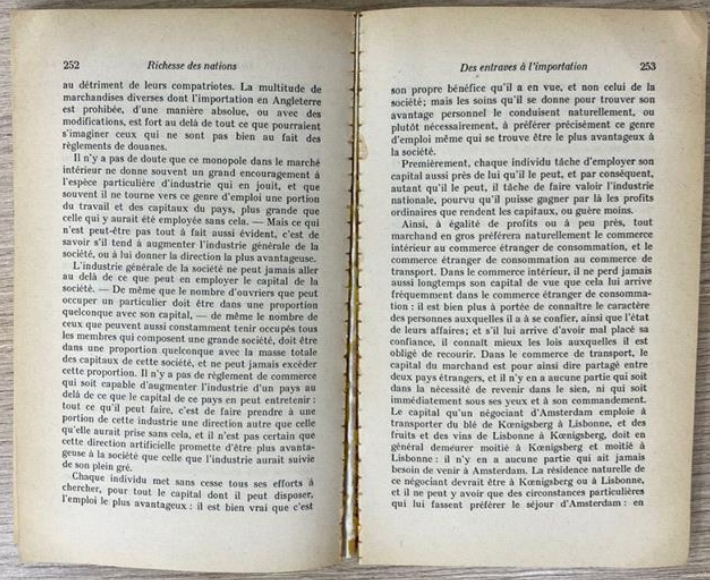
\includegraphics[scale=.7]{figura2.png}
        \label{figura2}
\end{figure}

\begin{figure}[H]
    \centering
    \caption{Riscos}
    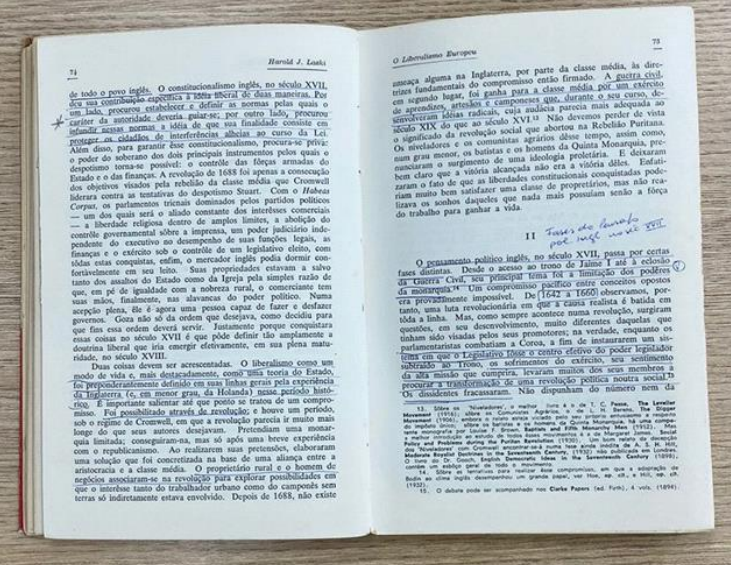
\includegraphics[scale=.7]{figura3.png}
        \label{figura3}
\end{figure}

Sendo este o grupo 3, ficamos responsáveis pela Classe 2  —  Religião  —  da Biblioteca Central da Universidade de Brasília (\textbf{BCE}).

Sem o cadastro de livros a serem pesquisados, o plano amostral mais indicado seria o conglomerado em dois estágios \cite{cochran1977sampling}, mas o trabalho foi feito como se fosse um plano aleatório simples ou estratificado, seguindo o esquema a seguir: 

Fomos à biblioteca verificar primeiramente quantas estantes existem em sua classe correspondente. No caso, haviam apenas duas estantes para esta classe, a qual dividimos em 4 (frente e verso). A seguir, usando os números aleatórios de uma página específica recebida do livro “A Million Random Digits with 100000 Normal Deviates” \cite{rand1955million}, cada componente do grupo selecionou 1 (uma) estante a ser pesquisada. Os membros do grupo  garantiram que a mesma estante não foi utilizada mais de uma vez. 

Como o tamanho das prateleiras era diferente para cada membro do grupo, utilizou-se critérios específicos para estimar o número total de livros para antes de realizar o sorteio. Para a prateleira 4, a menor de todas, a medida adotada foi de contar o número total de livros para obter o parâmetro, que é $N = 196$; e posteriormente sortear deste N total um $n=25$ amostras, sorteadas segundo a tabela de números aleatórios \cite{rand1955million} na página 265, linha 13.225. % Favor cada membro inserir aqui sua metogolodia de contagem do N, página e linha utilizada da tabelinha para fazer a seleção de amostras.

\section{Referencial teórico}

A amostragem é uma técnica estatística que permite conseguir resultados aproximados para a população a partir de uma quantidade menor de informações, ou seja, por meio de observações de apenas um "pedaço"$\:$dessa população. Dessa forma, consegue-se, com um intervalo de confiança, reduzir os custos e otimizar o tempo de coleta de informações sem perder a credibilidade para o estudo em questão.

\subsection{Amostragem Aleatória Simples}
Na amostragem aleatória simples, cada componente da população tem a mesma probabilidade de ser selecionado para fazer parte da amostra, ou seja, dada uma população com $N$ indivíduos, cada um possui probabilidade igual a $\displaystyle \frac{1}{N}$ de ser selecionado. Além disso, é necessário que a seleção de indivíduos seja feita de forma aleatória.

Quando a amostra é relativamente grande, o Teorema do Limite Central garante que a média amostral ($\bar{X}$) aproxima-se de uma distribuição normal com média $\mu$ e variância $\sigma^2/n$, e o tamanho necessário de amostra (n'), para um determinado erro $\varepsilon$, nível de confiança $\gamma$ e população infinita, é dado pela seguinte expressão:
{\large $$n'=\frac{z^2_\frac{\alpha}{2} \times s^2}{\varepsilon^2}$$} 
Com:
\begin{itemize}
\item $z_\frac{\alpha}{2}$: quantil da distribuição normal padrão e aproximadamente igual a 1,96 para $\alpha$ = 5\% e 1,64 para $\alpha$ = 10\%
\item $\alpha$: nível de significância, equivale a $1-\gamma$
\item $s^2$: variância amostral da variável analisada
\item $\varepsilon$: erro sobre a estimativa do parâmetro populacional
\item $\mu$: média populacional da variável analisada
\item $\sigma^2$: variância populacional da variável analisada
\end{itemize}

O erro $\varepsilon$ significa que, se fosse possível construir uma grande quantidade de intervalos de confiança da forma $\bar{X}-\varepsilon \leq \mu \leq \bar{X}+\varepsilon$, todos baseados em amostras independentes de tamanho n', $100 \times \gamma\%$ (em geral, 90\% ou 95\%) conteriam o parâmetro populacional $\mu$.

Quando se conhece o tamanho da população (N), o valor de n' pode ser corrigido para se reduzir o tamanho necessário de amostra para:
{\large $$n=\frac{n'N}{N+n'}$$}
É importante ressaltar que, como a proporção pode ser escrita como a média de variáveis indicadoras, os resultados apresentados acima também são válidos. Além disso, caso não se conheça o valor verdadeiro da variância, pode-se utilizar uma cota superior de 0,25, pois este é o valor máximo da variância de uma variável indicadora. \cite{cochran1977sampling}

\subsubsection{Estimativa de parâmetros}

A média amostral é dada por:

$$\bar{x}=\sum^n_{i=1}\frac{x_i}{n}$$

A média amostral é um estimador não viesado para a média populacional (FALCÃO,2013,p.5 \cite{joao} apud COCHRAN,1977 \cite{cochran1977sampling})

A variância para uma amostra aleatória simples com reposição ($AAS_c$) é dada por (FALCÃO,2013,p.5 \cite{joao} apud COCHRAN,1977 \cite{cochran1977sampling}):  

$$\sigma^2 = \frac{\sum^N_{i=1}(x_i-\bar{X})^2}{N}$$

Ainda segundo FALCÃO,2013,p.5 \cite{joao} apud COCHRAN,1977 \cite{cochran1977sampling}, a variância para uma amostra aleatória simples sem reposição ($AAS_s$) é dada por:

$$S^2=\frac{\sum^N_{i=1}(x_i-\bar{X})^2}{N-1}$$

Sendo assim, definem-se as variâncias da média $\bar{x}$ como (FALCÃO,2013,p.5 \cite{joao} apud COCHRAN,1977 \cite{cochran1977sampling}):

$$Var_{AAS_c}(\bar{x})=\frac{S^2}{n}\frac{(N-n)}{N} = \frac{S^2}{n}(1-f)$$

onde $f$ é dado por $\frac{n}{N}$.

Essa proporção inserida na fórmula é conhecida como fator de Correção para
População Finita (CPF), ou do inglês Finite Population Correction (FPC) (FALCÃO,2013,p.5 \cite{joao} apud COCHRAN,1977 \cite{cochran1977sampling}).

É válido observar que para o cálculo dessa variância é preciso conhecer previamente alguns parâmetros populacionais tais como seu tamanho e a média de seus valores. Na prática, tais parâmetros não podem ser conhecidos, mas podem ser estimados a partir dos dados amostrais (FALCÃO,2013,p.5 \cite{joao} apud COCHRAN,1977 \cite{cochran1977sampling}).

De acordo com Cochran (FALCÃO,2013,p.5 \cite{joao} apud COCHRAN,1977 \cite{cochran1977sampling})), um estimador não viciado da variância populacional estimada $S^2$ ou $\sigma^2$ é dado por:

$$\widehat{Var}(\bar{x})=\frac{\sum^n_{i=1}(x_1-\bar{x})^2}{n-1}=s^2$$

\newpage

\section{Análises}

\subsection{Análise exploratória}

\subsubsection{Avaria}

\begin{figure}[H]
    \centering
    \caption{Gráfico de setores da proporção de livros avariados}
    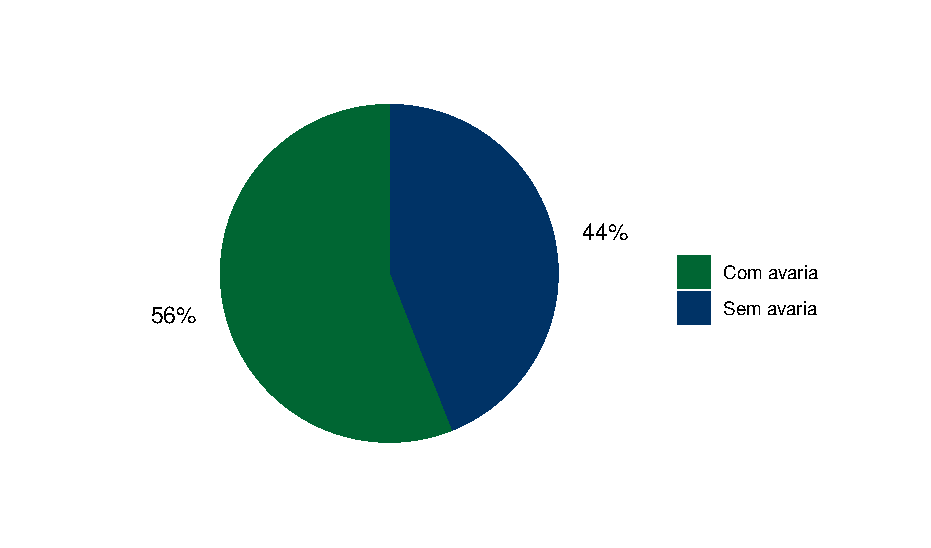
\includegraphics[scale=1]{grafico2.pdf}
\end{figure}

\newpage

\subsubsection{Avaria por prateleira}

\begin{figure}[H]
    \centering
    \caption{Gráfico de barras da quantidade de avaria pela prateleira}
    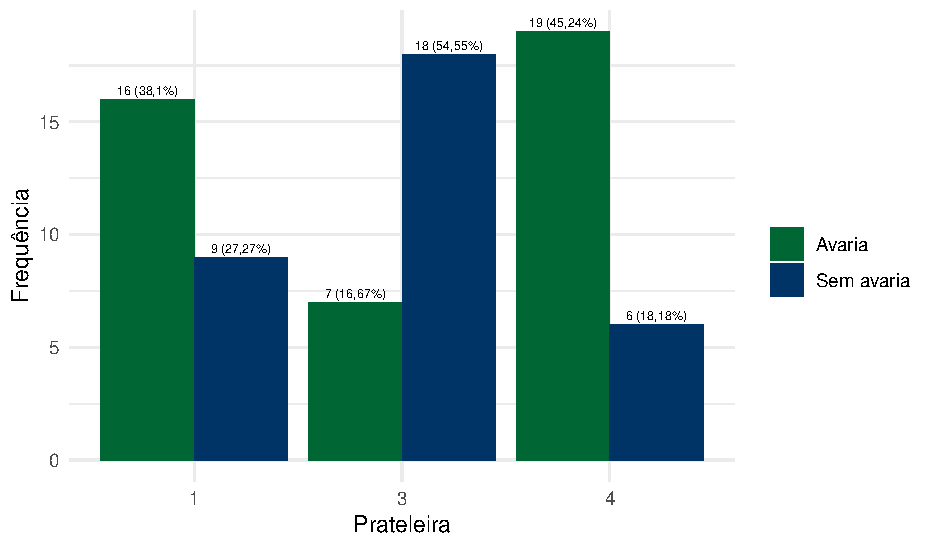
\includegraphics[scale=1]{grafico5.pdf}
\end{figure}

\begin{figure}[H]
    \centering
    \caption{Diagrama de Sankey da proporção de livros avariados pela prateleiras}
    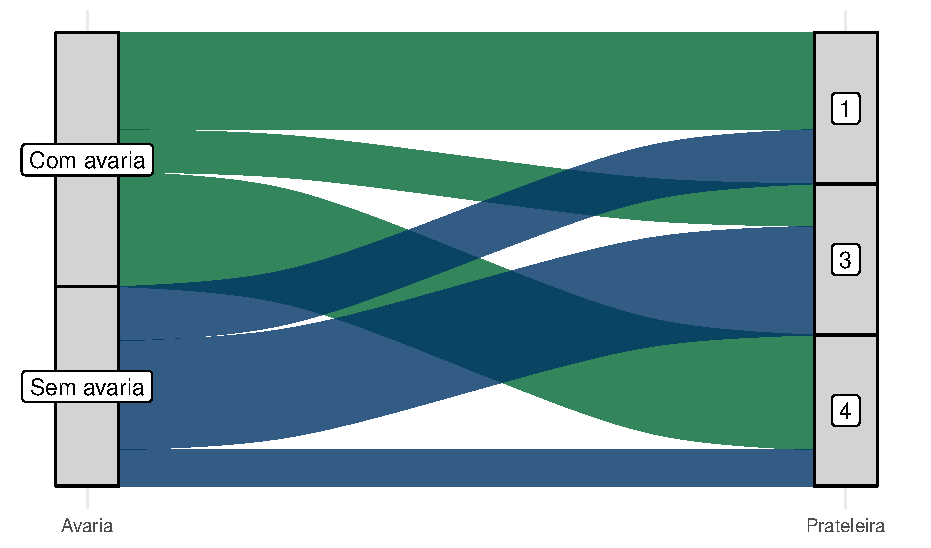
\includegraphics[scale=1]{grafico9.pdf}
\end{figure}

Testaremos a hipótese de que a quantidade de avarias difere entre as prateleiras.

$$\begin{cases}
H_0 : \mbox{As médias de livros avariados das prateleiras são iguais}\\
H_1 : \mbox{Existe pelo menos uma prateleira com média diferente}
\end{cases}$$\\

\begin{table}[H]
\centering
\begin{tabular}{c|ccccc}
\hline
\begin{tabular}[c]{@{}c@{}}Fonte de \\ Variação\end{tabular} & \begin{tabular}[c]{@{}c@{}}Graus de \\ Liberdade\end{tabular} & \begin{tabular}[c]{@{}c@{}}Soma de \\ Quadrados\end{tabular} & \begin{tabular}[c]{@{}c@{}}Quadrado\\  Médio\end{tabular} & Estatística F & P-valor \\ \hline
Prateleiras & 2 & 3,12 & 1,56 & 7,31 & 0,0013 \\
Resíduos & 72 & 15,36 & 0,21 & & \\ \hline
Total & 74 & 18,48 & & & \\ \hline
\end{tabular}
\end{table}

Sob um nível de significância $\alpha = 5\%$, rejeitamos a hipótese nula $H_0$ de igualdade de médias de avarias nas prateleiras. Ou seja, ao menos uma prateleira difere em relação a quantidade de livros avariados.

Devemos verificar os pressupostos do teste ANOVA.

\newpage

\paragraph{Independência} 
\hfill \break
Testaremos a independência pelo gráfico de dispersão dos resíduos.

\begin{figure}[H]
    \centering
    \caption{Gráfico dos resíduos da ANOVA}
    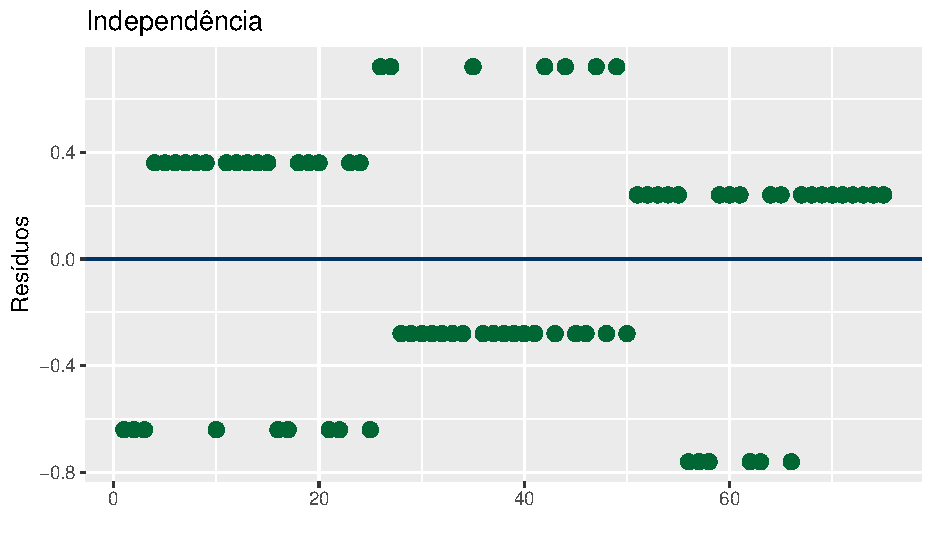
\includegraphics[scale=1]{grafico7.pdf}
\end{figure}

Por este gráfico, não podemos concluir pela independência dos resíduos, pois estes formam padrões lineares no gráfico de dispersão.

\newpage

\paragraph{Normalidade}

$$\begin{cases}
H_0 : \mbox{Os resíduos seguem distribuição normal}\\
H_1 : \mbox{Os resíduos não seguem distribuição normal}
\end{cases}$$\\

\begin{quadro}[H]
\centering
\caption{P-valor do teste de Shapiro-Wilk para normalidade dos resíduos}
\begin{tabular}{|c|c|c|}
\hline
\textbf{Variável} & \textbf{Teste Shapiro-Wilk} & \textbf{Decisão do teste} \\ \hline Resíduos ANOVA
 & \textless 0,001       & Rejeita $H_0$  \\ \hline  
\end{tabular}
\end{quadro}

\begin{figure}[H]
    \centering
    \caption{Gráfico Q-Q dos resíduos da ANOVA}
    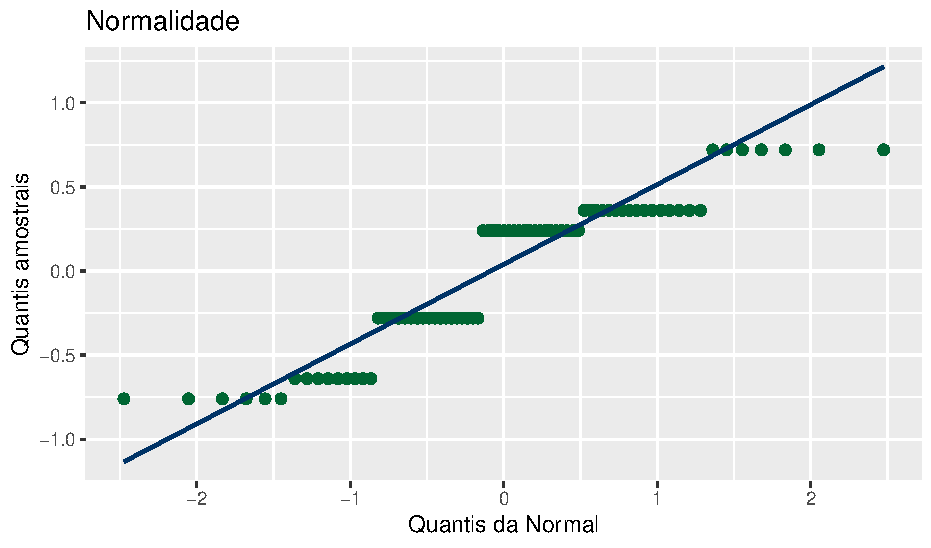
\includegraphics[scale=1]{grafico6.pdf}
\end{figure}

Pelo teste de Shapiro-Wilk e pelo Gráfico Q-Q, concluímos que os resíduos não seguem distribuição normal

\newpage

\paragraph{Homocedasticidade}
\hfill \break
Como os resíduos não seguem distribuição normal, faremos o teste de Levene para homocedasticidade, em detrimento do teste de Bartlett, este muito sensível a normalidade.

$$\begin{cases}
H_0 : \mbox{As variâncias das prateleiras são homogêneas}\\
H_1 : \mbox{Ao menos uma prateleira contém variância heterogênea}
\end{cases}$$\\

\begin{quadro}[H]
\centering
\caption{P-valor do teste de Levene para homocedasticidade}
\begin{tabular}{|c|c|c|}
\hline
\textbf{Variável} & \textbf{Teste de Levene} & \textbf{Decisão do teste} \\ \hline Variâncias das prateleiras
 &  0,647       & Não rejeita $H_0$  \\ \hline  
\end{tabular}
\end{quadro}

Pelo teste de Levene e Gráfico dos resíduos pelos valores ajustados, concluímos pela não rejeição de $H_0$, ou seja, as variâncias são homogêneas.

\begin{figure}[H]
    \centering
    \caption{Gráfico dos resíduos pelos resíduos ajustados da ANOVA}
    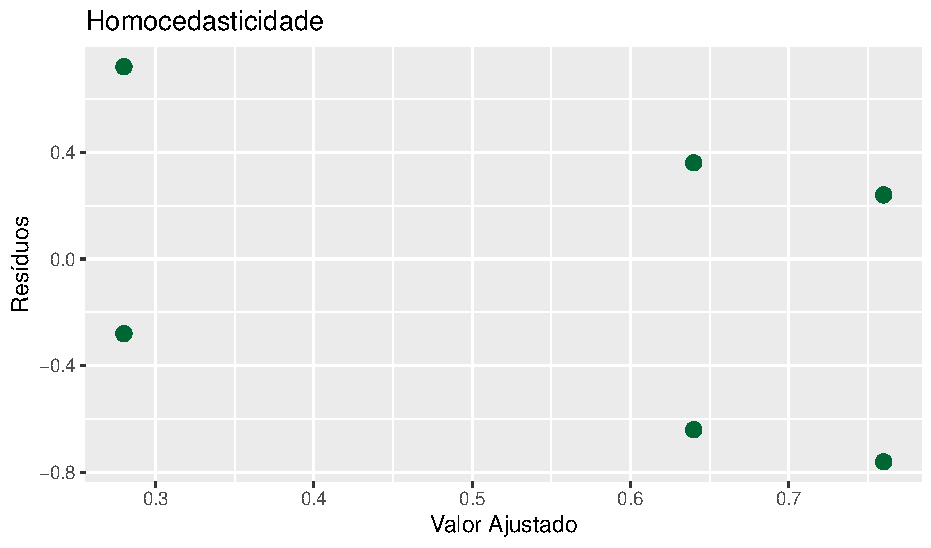
\includegraphics[scale=1]{grafico8.pdf}
\end{figure}

\newpage

Rejeitados alguns dos pressupostos, devemos portanto utilizar uma abordagem não paramétrica para testar a hipótese da diferença das médias de avarias nas prateleiras. Utilizaremos o teste de Kruskall-Wallis.

$$\begin{cases}
H_0 : \mbox{As medianas de livros avariados das prateleiras são iguais}\\
H_1 : \mbox{Existe pelo menos uma prateleira com mediana diferente}
\end{cases}$$\\

\begin{quadro}[H]
\centering
\caption{P-valor do teste de Kruskall-Wallis}
\begin{tabular}{|c|c|c|}
\hline
\textbf{Variável} & \textbf{Teste Kruskall-Wallis} & \textbf{Decisão do teste} \\ \hline Resíduos ANOVA
 & 0.002       & Rejeita $H_0$  \\ \hline  
\end{tabular}
\end{quadro}

Pelo teste de Kruskall-Wallis, concluímos que existem diferenças entre as medianas de avarias nas prateleiras.

\newpage

\subsubsection{Tipos de avaria}

\begin{figure}[H]
    \centering
    \caption{Gráfico de setores do tipo de avaria}
    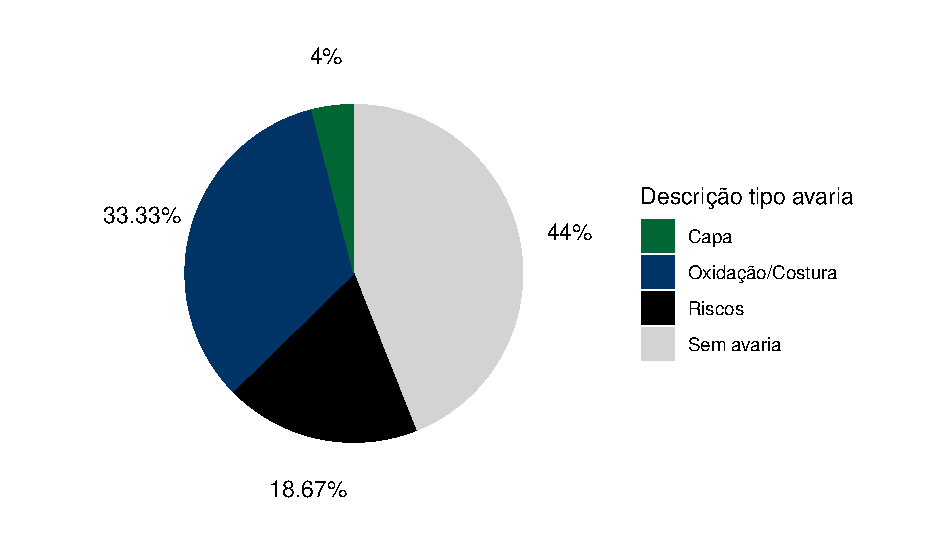
\includegraphics[scale=1]{grafico3.pdf}
\end{figure}

\begin{figure}[H]
    \centering
    \caption{Gráfico de setores do tipo de avaria}
    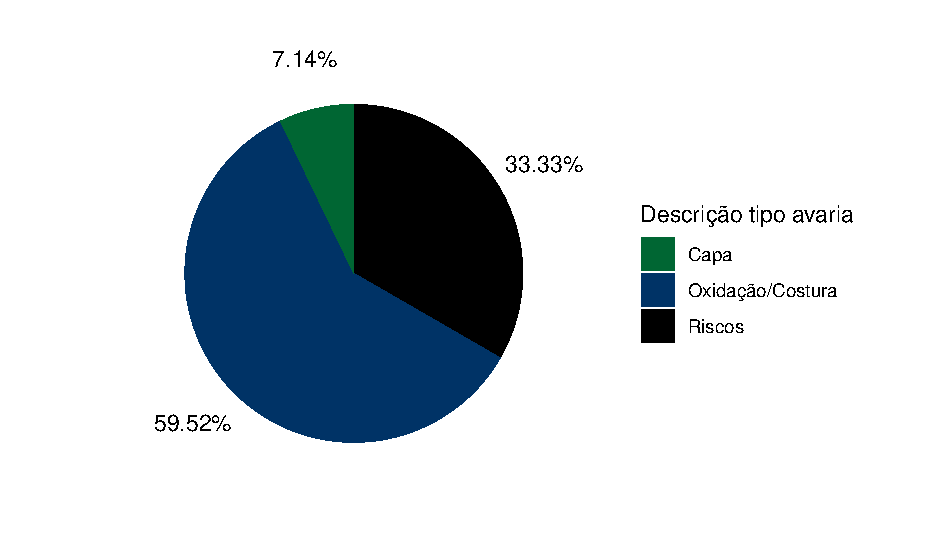
\includegraphics[scale=1]{grafico4.pdf}
\end{figure}

\newpage

\subsubsection{Tipo de avaria por prateleira}

\begin{figure}[H]
    \centering
    \caption{Gráfico de barras do tipo de avaria pela prateleira}
    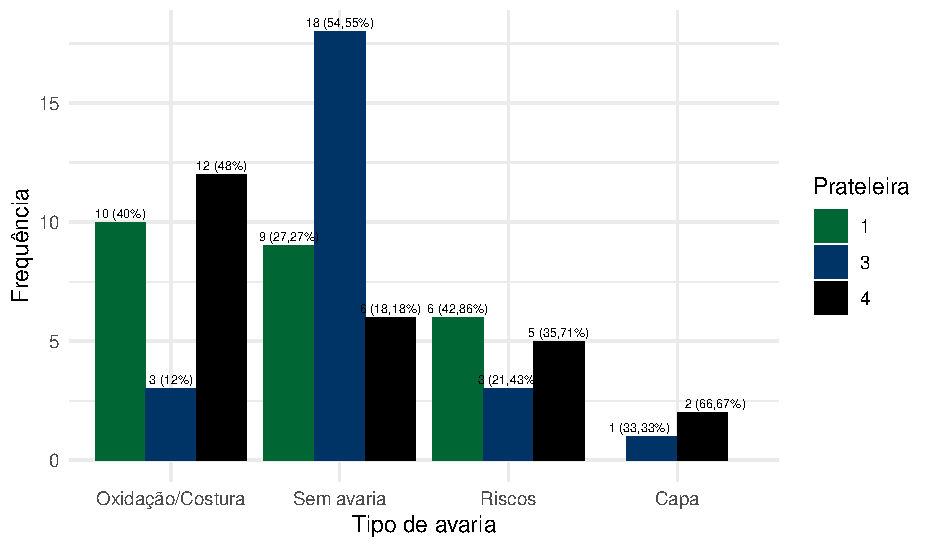
\includegraphics[scale=1]{grafico1.pdf}
\end{figure}

\begin{table}[H]
\centering
\caption{Frequências dos tipos de avaria pela prateleira}
\begin{tabular}{l|ccc|c}
\hline
\textbf{Tipos de avaria} & \textbf{Prateleira 1} & \textbf{Prateleira 3} & \textbf{Prateleira 4} & \textbf{Total} \\ \hline
Capa                 & 0 & 1 & 2 & 3 \\
Oxidação/Costura & 10 & 3 & 12 & 25 \\
Riscos                & 6 & 3 & 5 & 14 \\ \hline
\textbf{Total}      & 16 & 7 & 19 & 42 \\ \hline
\end{tabular}
\end{table}

Faremos um teste para testar a hipótese do tipo de avaria ter relação com a prateleira no qual o livro se encontra.

$$\begin{cases}
H_0 : \mbox{O tipo de avaria é independente da prateleira ao qual o livro se encontra}\\
H_1 : \mbox{Existe dependência do tipo de avaria à prateleira em que o livro se encontra}
\end{cases}$$\\

\begin{quadro}[H]
\centering
\caption{P-valor do teste Qui-Quadrado de independência}
\begin{tabular}{|c|c|c|}
\hline
\textbf{Variável} & \textbf{Teste Qui-quadrado} & \textbf{Decisão do teste} \\ \hline Tipo de avaria
 & 0,576       & Não rejeita $H_0$  \\ \hline  
\end{tabular}
\end{quadro}

Pelo teste Qui-quadrado, concluímos que não existe relação entre o tipo de avaria e a prateleira em que o livro se encontra.

\subsection{Amostragem}

Com base nas fórmulas referenciadas no referencial teórico, estimamos a verdadeira proporção de livros avariados na população.

Com estatística pontual $p=0,56$ e erro padrão $EP = 0,0573$, inferimos sobre o intervalo de confiança $\alpha = 5\%$ assintótico para a proporção em:

\begin{quadro}[H]
\centering
\caption{Intervalo de confiança para a proporção de livros avariados na população}
\begin{tabular}{|c|c|c|}
\hline
\textbf{Estatística pontual} & \textbf{Intervalo de Confiança (95\%)}                 \\ \hline
\begin{tabular}[c]{@{}c@{}}0,56\end{tabular} &    \begin{tikzpicture}[x=50]
       \draw (-0.2,0) -- (1.2,0);      
       \draw (0, 0) node[below=7pt] {$0,4477$};
       \draw[] (0,-0.1) -- (0,0.1);
       \draw (1, 0) node[below=7pt] {$0,6723$};       
       \draw[] (1,-0.1) -- (1,0.1);
   \end{tikzpicture} \\ \hline
\end{tabular}
\label{intervalo:media_x}
\end{quadro}

Aqui, não estamos fazendo correção de população finita, que deve ser posteriormente realizado caso o parâmetro $N$ seja conhecido.

\section{Conclusão}

\newpage

\section{Códigos Computacionais}

Confira na íntegra no \href{https://github.com/penasta/Amostragem/blob/main/scripts/analises.R}{Github}.


\begin{lstlisting}

if (!require("pacman")) install.packages("pacman")

pacman::p_load(
  tidyverse, data.table,
  readxl, readr, ggcorrplot, cowplot,
  RColorBrewer, scales, nortest, xlsx,
  skimr,xtable
  )

windowsFonts(Arial=windowsFont("sans"))

options(scipen=999)

# Definindo paleta de cores da UnB
cores_unb <- c("#006633", "#003366","#000000","lightgray")

percent <- function(absolute, digits = 2) {
  return(round(100 * absolute / sum(absolute), digits))
}

# Definindo função que retorna banco de dados com frequências
# relativas e absolutas de uma variável categórica
vector_frequencies <- function(vector) {
  frequency <- vector %>%
    table() %>%
    as_tibble() %>%
    mutate(
      rel = n %>%
        percent() %>%
        paste("%", sep = "")
    )
  colnames(frequency) <- c("groups", "absolute", "relative")
  return(frequency)
}

# 1.1 Dados ----
df <- read_excel("banco/grupo3.xlsx",
                     col_types = c("skip",
                                   "text", "text", "text","text",
                                   "text","text", "text", "text"))

# 1.2 ETL ----
colnames(df)
df$Classe <- factor(df$Classe)
df$Avaria <- as.numeric(df$Avaria)
df$Descrição_avaria <- factor(df$Descrição_avaria)
df$Tipo_avaria <- factor(df$Tipo_avaria)
df$Descrição_tipo_avaria <- factor(df$Descrição_tipo_avaria)
df$Prateleira <- factor(df$Prateleira)

# 2 Análises ----
# 2.0 Exploratória ----
# 2.0.1 Tabela completa em LaTeX ----
p_load(xtable)
xtable(df)

# 2.0.2 Tabela de contingência do tipo de avaria pela prateleira - LaTeX ----
xtable(table(df$Descrição_tipo_avaria,df$Prateleira))

# 2.0.3 Gráfico: Tipo de avaria pela prateleira ----
df$Descrição_tipo_avaria <- as.character(df$Descrição_tipo_avaria)
df %>%
  select(Descrição_tipo_avaria, Prateleira) %>%
  mutate(Descrição_tipo_avaria = ifelse(is.na(Descrição_tipo_avaria), "Sem avaria", Descrição_tipo_avaria)) %>%
  group_by(Descrição_tipo_avaria, Prateleira) %>%
  summarise(freq = n()) %>%
  mutate(
    freq_relativa = freq %>% percent(),
    porcentagens = str_c(freq_relativa, "%") %>% str_replace("\\.", ","),
    legendas = str_squish(str_c(freq, " (", porcentagens, ")"))
    ) %>%
  ggplot() +
  aes(
    x = fct_reorder(Descrição_tipo_avaria, freq, .desc = T),
    y = freq,
    fill = Prateleira,
    label = legendas
    ) +
  geom_col(position = position_dodge2(preserve = "single", padding = 0)) +
  geom_text(
    position = position_dodge(width = .9),
    vjust = -0.5, hjust = 0.5,
    size = 2) +
  scale_fill_manual(values = cores_unb)+
  labs(x = "Tipo de avaria", y = "Frequência") +
  theme_minimal()
ggsave("resultados/grafico1.pdf", width = 158, height = 93, units = "mm")


# 2.0.4 Proporção avaria ----

contagem2 <- df %>%
  mutate(Descrição_avaria = ifelse(Descrição_avaria == "Sem avaria", "Sem avaria","Com avaria")) %>%
  group_by(Descrição_avaria) %>%
  summarise(Freq = n()) %>%
  mutate(Prop = round(100 * (Freq / sum(Freq)), 2)) %>%
  arrange(desc(Descrição_avaria)) %>%
  mutate(posicao = cumsum(Prop) - 0.5 * Prop,
         ymax = cumsum(Prop),
         ymin = c(0, head(ymax, n=-1)))

ggplot(contagem2) +
  aes(
    x = factor(""),
    y = Prop,
    fill = factor(Descrição_avaria)
  ) +
  geom_bar(width = 1, stat = "identity") +
  coord_polar(theta = "y") +
  scale_fill_manual(values = cores_unb,name = "") +
  theme_void() +
  geom_text(
    aes(x = 1.8, y = posicao, label = paste0(Prop, "%")),
    color = "black"
  )
ggsave("resultados/grafico2.pdf", width = 158, height = 93, units = "mm")


# 2.0.5 Proporção tipo de avaria ----
contagem <- df %>%
  mutate(Descrição_tipo_avaria = ifelse(is.na(Descrição_tipo_avaria), "Sem avaria", Descrição_tipo_avaria)) %>%
  group_by(Descrição_tipo_avaria) %>%
  summarise(Freq = n()) %>%
  mutate(Prop = round(100 * (Freq / sum(Freq)), 2)) %>%
  arrange(desc(Descrição_tipo_avaria)) %>%
  mutate(posicao = cumsum(Prop) - 0.5 * Prop,
         ymax = cumsum(Prop),
         ymin = c(0, head(ymax, n=-1)))

ggplot(contagem) +
  aes(
    x = factor(""),
    y = Prop,
    fill = factor(Descrição_tipo_avaria)
  ) +
  geom_bar(width = 1, stat = "identity") +
  coord_polar(theta = "y") +
  scale_fill_manual(values = cores_unb,name = "Descrição tipo avaria") +
  theme_void() +
  geom_text(
    aes(x = 1.8, y = posicao, label = paste0(Prop, "%")),
    color = "black"
  )
ggsave("resultados/grafico3.pdf", width = 158, height = 93, units = "mm")

# 2.0.6 Proporção tipo de avaria - tirando "sem avaria" ----
contagem3 <- df %>%
  na.omit() %>%
  group_by(Descrição_tipo_avaria) %>%
  summarise(Freq = n()) %>%
  mutate(Prop = round(100 * (Freq / sum(Freq)), 2)) %>%
  arrange(desc(Descrição_tipo_avaria)) %>%
  mutate(posicao = cumsum(Prop) - 0.5 * Prop,
         ymax = cumsum(Prop),
         ymin = c(0, head(ymax, n=-1)))

ggplot(contagem3) +
  aes(
    x = factor(""),
    y = Prop,
    fill = factor(Descrição_tipo_avaria)
  ) +
  geom_bar(width = 1, stat = "identity") +
  coord_polar(theta = "y") +
  scale_fill_manual(values = cores_unb,name = "Descrição tipo avaria") +
  theme_void() +
  geom_text(
    aes(x = 1.8, y = posicao, label = paste0(Prop, "%")),
    color = "black"
  )
ggsave("resultados/grafico4.pdf", width = 158, height = 93, units = "mm")


# 2.1 Proporção estimada na população, com intervalo de confiança; estatística pontual e erro padrão. ----
p_load(samplingbook)
Sprop(y=df$Avaria)

# 2.1.1 Mesmo, porém "chutando" um valor para N ----
# N = População de livros na Classe 2 - Religião - na BCE.
Sprop(y=df$Avaria,N=197+2*1500)

# 2.2.1 Verificando se a avaria pode ser explicada pelo tipo da avaria + qual prateleira o livro foi coletado
summary(aov(Avaria ~ Tipo_avaria + Prateleira,data=df)) # Não significativo

# 2.2.2 Verificando se a avaria pode ser explicada por qual prateleira o livro foi coletado ----
anova = aov(Avaria ~ Prateleira,data=df)
summary(anova) # O teste anova indica que a prateleira em que o livro foi encontrado pode explicar o tipo de avaria.
# Pressupostos do teste

# 2.2.2.1 Normalidade dos resíduos ----
shapiro.test(anova$residuals) # Não são normais
qqnorm(anova$residuals)
qqline(anova$residuals)

# 2.2.2.2 Independência ----
plot(anova$residuals)
plot(anova$residuals~anova$fitted.values)
# Não aparentam ser independentes

# 2.2.2.3 Homocedasticidade ----
pacman::p_load(car)
leveneTest(y=df$Avaria,group=df$Prateleira)
# Variâncias homogêneas.

# 2.2.3 Teste não paramétrico - Kruskall-Wallis ----
kruskal.test(Avaria ~ Prateleira,data=df) # Pelo teste não paramétrico de Kruskall-Wallis, concluímos que existem diferenças entre a quantidade de avarias nas prateleiras.

# 2.2.4 Verificando se o tipo de avaria é homogêneo entre as prateleiras
p_load(stats)
chisq.test(df$Tipo_avaria,df$Prateleira
#           , simulate.p.value = TRUE,B=10000
           )
# O teste qui-quadrado indica que O tipo de avaria é independente da prateleira (H0 não rejeitado).

# 2.2.5 Diagrama de Sankey: Proporção de livros avariados/não avariados por cada prateleira ----

p_load(ggalluvial)
prop <- df |>
  select(Descrição_avaria,Prateleira) |>
  count(Descrição_avaria, Prateleira) |>
  mutate(proptot = prop.table(n),
         Descrição_avaria = ifelse(Descrição_avaria == "Avaria","Com avaria","Sem avaria"))

ggplot(as.data.frame(prop),
       aes(y = proptot, axis1 = factor(Descrição_avaria), axis2 = factor(Prateleira))) +
  geom_alluvium(aes(fill = factor(Descrição_avaria)), width = 1/12,alpha=.8,show.legend = FALSE) +
  geom_stratum(width = 1/12, fill = cores_unb[4], colour = cores_unb[3],alpha=1) +
  geom_label(stat = "stratum", infer.label = TRUE) +
  scale_x_discrete(limits = c("Avaria", "Prateleira"),
                   expand = c(.05, .05),
                   labels = c("Avaria", "Prateleira")) +
  scale_fill_manual(values = cores_unb) +
  scale_y_continuous(labels = NULL,
                     name = NULL,
                     breaks = NULL) +
  theme_minimal()


# 2.2.6 Diagrama de Sankey: Tipo de avaria por cada prateleira ----

prop2 <- df |>
  select(Descrição_tipo_avaria,Prateleira) |>
  mutate(Descrição_tipo_avaria = ifelse(is.na(Descrição_tipo_avaria), "Sem avaria", Descrição_tipo_avaria)) %>%
  count(Descrição_tipo_avaria, Prateleira) |>
  mutate(proptot = prop.table(n))

ggplot(as.data.frame(prop2),
       aes(y = proptot, axis1 = factor(Descrição_tipo_avaria), axis2 = factor(Prateleira))) +
  geom_alluvium(aes(fill = factor(Descrição_tipo_avaria)), width = 1/12,alpha=.8,show.legend = FALSE) +
  geom_stratum(width = 1/12, fill = cores_unb[4], colour = cores_unb[3],alpha=1) +
  geom_label(stat = "stratum", infer.label = TRUE) +
  scale_x_discrete(limits = c("Avaria", "Prateleira"),
                   expand = c(.05, .05),
                   labels = c("Avaria", "Prateleira")) +
  scale_fill_manual(values = rev(cores_unb)) +
  scale_y_continuous(labels = NULL,
                     name = NULL,
                     breaks = NULL) +
  theme_minimal()

\end{lstlisting}


\newpage

\printbibliography 

\end{document}